\section{Basis-begreber??}

En spole er en noget der bliver brugt til mange forskellige ting, men det spolen bruges til er, at der sendes strøm igennem spolen, når strømen er blevet sendt igennem opstår der et magnetfelt om spolen. Mag-netfeltet der bliver dannet omkring spolen, vil ligne det fra en magnet, men skal være af samme form så spolen. Feltet bliver meget kraftigere hvis der er jern inde i spolen. 

Hvis spolen kortsluttes mens der er strøm der løber igennem, vil spolen på bedst muligvis forsøge at op-retholde strømmen, men da strømmen ikke kan løbe i en kreds kan det ikke lade sig gøre for spolen og opretholde strømmen.  Strømmen bruges i stedet i feltet, det vil sige at spændingen over spolens ender stiger voldsomt og der opstår ofte en gnist. Det er det samme der sker i tænd spolen i bilen eller i et køk-kenapparat eller lignende.

\begin{figure}[htbp]
	\centering
	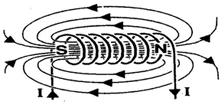
\includegraphics[width=1\textwidth]{Vildledning/Schematics/magnetfelt_omkring_en_spole.png}
	\caption{Magnetfelt omkring en spole.\cite{spoler}}
	\label{spole1}
\end{figure}

En magnet der er permanent er også en metalgering, som der ofte er jern i, magneten for derved den egenskab, at den bliver magnetisk.  Bliver en permanent magnet skubbet over til noget der er kortslutte-de, det kan være en spole sker der det, at den permanente magnet vil fremkalde strøm i spolen, når der er fremkaldt en strøm vil den permanente magnet forsøge, at holde feltet ude. Det betyder at spolen forsøger, at lave poler, som vil vende modsat af den permanente magnet. Men strømen vil i løbet af me-get kort tid forsvinde, hvis magneten ligger stille dette skyldes, at energien/strømen vil blive omdannet til varme inde i spolens ohmske modstand. Hvis magneten derimod bliver fjernet sker der omvendte, altså vil den påbegynde i det modsat retning, altså starte fra det felt der var inden magneten blev tilføjet. Ud fra dette kan det konkluderes, at der kun er strøm i spolen når der enten sættes et batteri til eller mag-netfeltet ændres. Hvis feltet forbliver konstant vil strømen forsvinde hurtigt og gå i nul dette skyldes også den ohmske modstand. 

En spole har ud fra dette altså ingen magnetfelt, medmindre den bliver påvirket af strøm eller man påvir-ker den vedhjælp af magnetisme. 

Der findes en række stoffer ved lave temperaturer disse stoffer er superledende, som også betyder, at de ingen elektrisk modstand har, når de ingen elektrisk modstand har ligger modstanden på 0 ohm. Der er tale om legeringer af stoffer der er sjældne, men er almindlig kendte i blandt andet bly og kviksølv. Laves der en blyring, bly ringen bliver sat ved stuetemperatur hvor der bliver sat en permanent magnet igen-nem, hvis nu det hele bliver kølet ned til det absolutte nulpunkt som ca. er -273C, når dette er gjort fjer-nes den permanente magnet, når den permanente magnet er blevet fjernet vil der ske det, som normalt sker ved induktion der vil nemlig opstå en strøm i blyringen, den strøm der opstår vil sørger for og gen-skabe det magnetfelt, som den permanente magnet havde. Der er ingen modsat hvilket også vil gøre, at strømmen vil forsætte så der haves et konstant magnetfelt, som er magen til det oprindelige magnetfelt. Magnetfeltet bliver målt i en enhed kaldet Tesla, som er opkaldt efter Nikola Tesla 1856-1943. 


\subsection{Mikrobølger}

En metode man kan bruge til at sende energi trådløst er ved hjælp af mikrobølger hvor man så omdanner den elektriske energi til mikrobølger og så sender dem var en PTU (Power Transmitter Unit) og til PRU (Power Receiver Unit). Hvor ved at man så omdanner mikrobølgerne tilbage til elektrisk strøm. Den typiske frekvens man bruger ligger mellem 300 MHZ og 300 GHZ. Mikrobølger har en fordel i form af at de kan sammen med at de sender energi, så kan de også bruges til at sende information, altså de kan bruges til kommunikation.  Det er ikke en mulighed som bliver brugt særlig ofte, da der kan ske mutationer hvis man er udsat for enten for hård stråling eller hvis man ofte bliver udsat for strålingen. Der er så stor fare at The Federal Communications Commission (FCC) har beslaglagt de stærke transmittere. Det er en af grundene til at man ikke bruger dem i bl.a. mobilopladere. FCC har lagt restriktioner på laderne til at må være på maks 4 W.

\subsection{Elektromagnetisme}
Elektromagnetisme er i sin enkelthed meget simpel. Elektromagnetisme virker på den måde at man har et materiale som man gør magnetisk ved hjælp af at sende en elektrisk strøm igennem. Ved at man gør det vender atomerne sig så de følger strømmen, og man får derved skabt 2 modstående poler som tiltrækker negativt eller positivt ladede partikler. En af fordele ved elektromagnetisme er at man selv kan sørge for hvornår et materiale skal være magnetisk og hvornår materialet ikke skal være magnetisk, ved at det er elektrisk kan man også bruge det til at vende polerne. Hvis man bruger jævnstrøm kan man holder polerne på plads, og hvis man bruger vekselstrøm kan man få polerne til at skifte retning kan man styre magnetiske felter. Og det gør at man kan bruge dem som motor. Når man snakker om elektromagnetisme bliver man også nød til at snakke om induktion. Induktion sker når man bruger magnetisme til at vende polariteten på fx en gryde eller mobil. Man kan vende polariteten på en gryde for at gøre gryden varm, altså til at lave mad, men uden faren for at man kan brænde sig på blusset bagefter, da pladen aldrig er blevet varm. Man kan også bruge induktion til hvis man vil lade sin mobiltelefon op, der er efterhånden mange teleselskaber som har gjort deres mobiler klar til at kunne lades op uden at skulle sætte et stik i den ene ende. Det er fx selskaber som Apple, Samsung, Huawei osv. Måden telefonen lader er at telefonen ligges på en flade hvor der er et magnetisk felt, som telefonen bryder og når det sker begynder telefonen lige som gryden at modtage energi, som den omdanner til elektrisk energi.
%\subsection{Spoler}
%I dette afsnit er der planlagt, at blive snakket om spoler. Både i forhold til vores kredsløb i plecs, samt hvordan det bedst kan benyttes til "wireless power transfer".
\newpage
\subsection{Opbygning af kredsløb??}
\begin{figure}[htbp]
	\centering
	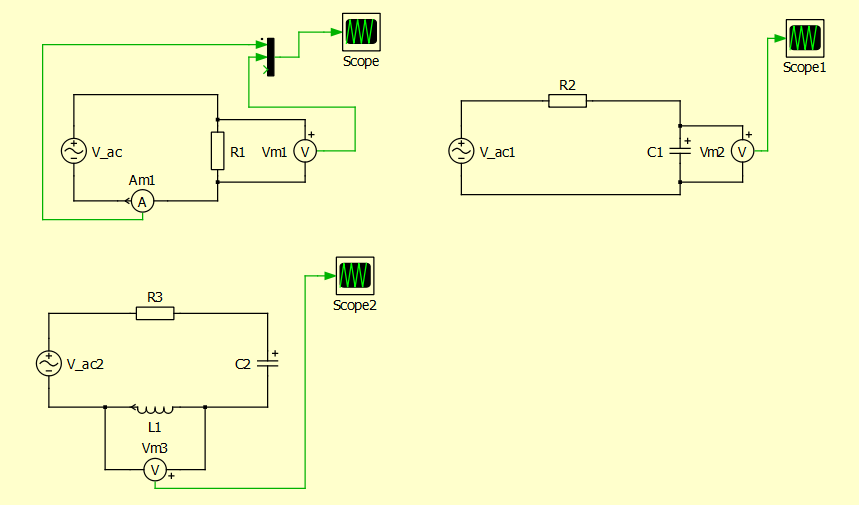
\includegraphics[width=1\textwidth]{Vildledning/Schematics/Eks1_LCR.png}
	\caption{LCR-Kredsløb}
	\label{forslag1}
\end{figure}

Hvor:
\begin{table}[H]
	\begin{tabular}{l|l}
	$R$     & Resistans [\si \ohm] \\
	$V_{ac}$ 	   &  Generator[\si Volt] \\
	$A$ 	   & Ampere-meter [\si Ampere] \\
	$V$			& Volt-meter [\si Volt]
	\end{tabular}
\end{table}
